\chapter{U/I/R-Messung und Messwerke}
\section{Einleitung}

\begin{table}[h]
	\centering
	\begin{tabular}{|c|c|}
		\hline 
		Teilnehmer 		& Oskar Fürnhammer, Katharina Kralicek, Patrick Mayr \\
		\hline 
		Datum 		& 26.11.2018 \\ 
		\hline 
		Messplatzbez. 	& CA0402-3 \\
		\hline
	\end{tabular} 
	%\caption{Grundlegende Information der 1. Laborübung}
\end{table}

\begin{table}[h]
	\centering
	\begin{tabular}{ c | c }

Gerät				& Bezeichnung		\\
\hline

Multimeter			& Agilent U1232A 		\\
Multimeter			& Agilent U1232A 		\\
Multimeter			& Neumann 9140	 	\\
Netzgerät			& Rigol DP832 		\\
Oszilloskop			& Keysight DSOX2002A 	\\
Funktionsgenerator		& Agilent U1232A 		\\

	\end{tabular}

	\caption{Verwendete Geräte}

\end{table}

\newpage

\section{Spannungs-, Strom- und Widerstandsmessung}

\subsection{Spannungsmessung}
\subsubsection{Berechnung des Innenwiderstandes des Voltmeters}
In der ersten Übung soll der Innenwiderstand des Voltmeters ermittelt werden. Die Schaltung zur Messung des Spannungswertes wird laut Abb. aufgebaut
~\\
TODO: SCHALTUNG		\\
~\\
Dieser Schaltung wurde mit einer Spannung $U$ von 10V versorgt. Der mit einem Ohmmeter gemessenen Widerstand $R_1$ ergab 100,2k$\Omega$. Die Spannung $U_V$ am Voltmeter betrug 9,90V.	\\
~\\
Die Spannung am Widerstand $R_1$ wird aus der Differenz von der Eingangsspannung und der Spannung am Voltmeter berechnet: 
\begin{equation}
	U_{R1} = U - U_V = 0,1V
	\label{eq:1}
\end{equation}
Der Strom durch $R_1$ ergibt sich als Quotient aus der berechneten Spannung und dem Widerstand $R_1$:
\begin{equation}
	I = \dfrac{U_{R1}}{R_1} = \dfrac{U - U_V}{R_1} = 0,998\mu A
\end{equation}
Der Innenwiderstand des Voltmeters $R_i$ wird aus den zuvor berechneten Spannung und Strom berechnet:
\begin{equation}
	R_i = \dfrac{U_V}{I} = 9,92M\Omega
\end{equation}
\begin{table}[h]
	\centering
	\begin{tabular}{|c|c|}
	\hline 
	Spannungsquelle $U [V]$			& 10 		\\ 
	\hline 
	Vorwiderstand $R_1 [k\Omega]$		& 100,2	\\ 
	\hline 
	Spannung an Voltmeter $U_V [V]$ 	& 9,90	\\ 
	\hline 
	Spannung am Widerstand $R_1 [V]$	& 0,1		\\ 
	\hline 
	Strom durch $R_1 [\mu A]$		& 998		\\ 
	\hline 
	Innenwiderstand $R_i [M\Omega]$	& 9,92	\\ 
	\hline 
	\end{tabular}
	\caption{Auswertung dieser Übung}
\end{table}
~\\
Der Innenwiderstand des Multimeters ist im MegaOhm-Bereich, damit der Strom, der durch das Messgerät fließt, klein ist, um die Spannungsmessung so gering wie möglich zu verfälschen.

\subsubsection{Bestimmung der Spannung am Multimeter}
Bei dieser Messung soll eruriert werden, wie sich die Spannungsmessung auf die Berechnung des Innenwiderstandes auswirkt.
~\\
TODO: SCHALTUNG		\\
~\\
Dieser Schaltung wurde mit einer Spannung $U$ von 10V versorgt. Der mit einem Ohmmeter gemessenen Widerstand $R_M$ ergab 100,2k$\Omega$. Die Spannungen $U_{V1}$ und $U_{V2}$ an den beiden Voltmetern betrugen 9,80V.	\\
~\\
Die beiden parallel geschalteten Voltmetern werden in der Berechnung durch einen Ersatz-Innenwiderstand ersetzt. Es wird angenommen, dass beide Ersatzwiderstände den selben Wert von $9,92 M\Omega$ haben.
\begin{equation}
	R_{iG} = \dfrac{R_{i1} \cdot R_{i2}}{R_{i1} + R_{i2}} = 4,96 M\Omega
\end{equation}
Die Spannung am Voltmeter V2 wird als Teilspannung mit Hilfe der Spannungsteilerregel berechnet:
\begin{equation}
	U_{V2} = U \cdot \dfrac{R_{iG}}{R_M + R_{iG}} = 9,80V
\end{equation}
\begin{table}[h]
	\centering
	\begin{tabular}{|c|c|}
	\hline 
	Spannungsquelle $U [V]$			& 10 		\\ 
	\hline 
	gemessene Spannung an Voltmeter $U_{V1} [V]$ 	& 9,80	\\ 
	\hline 
	gemessene Spannung an Voltmeter $U_{V2} [V]$ 	& 9,80	\\ 
	\hline 
	\end{tabular}
	\caption{Auswertung dieser Übung}
\end{table}

\subsubsection{Messbereichserweiterung}
Das Ziel dieser Teilübung ist, den Messbereichserweiterung der Spannungsmessung zu erstellen.
~\\
TODO: SCHALTUNG		\\
~\\
Dieser Schaltung wurde mit einer Spannung $U$ von 10V versorgt. Die Widerstände $R_M$ und $R_V$ wurde jeweils mit einem Ohmmeter gemessen und ergaben 99,5k$\Omega$ für $R_M$ bzw. 100,2k$\Omega$ für $R_V$. Die gemessene Spannung $U_{RM}$ an dem Widerstand $R_M$ betrug 4,952V.	\\
~\\
Der Faktor $f_{ME}$ der Messbereichserweiterung wird mit der Formel \ref{eq:me_spg} berechnet:
\begin{equation}
	f_{ME} = \dfrac{U}{U_{RM}}
	\label{eq:me_f}
\end{equation}
Die Eingangsspannung $U$ wird aus der Addition von der Spannung vom Widerstand $R_M$ und von der vom Vorwiderstand $R_V$ errechnet.
\begin{equation}
	U = U_V + U_{RM} = I \cdot R = I \cdot (R_V + R_M \parallel R_{i2})
	\label{eq:me_spg}
\end{equation}
Die Spannung $U_V$ am Vorwiderstand $R_V$ wird durch die folgende Formel berechnet:
\begin{equation}
	U_V = I \cdot R_V
\end{equation}
Die Spannung $U_{RM}$ am Widerstand $R_M$ wurde über das ohm'sche Gesetz berechnet:
\begin{equation}
	U_{RM} = I \cdot (R_M \parallel R_{i2})
	\label{eq:me_spg_rm}
\end{equation}
Das Voltmeter wird durch eine Ersatz-Innenwiderstand ersetzt, somit ergibt sich der Parallelwiderstand $R_P$
\begin{equation}
	R_P = \dfrac{R_M \cdot R_{i2}}{R_M + R_{i2}} = 98,5k\Omega
\end{equation}
Setzt man die Formeln \ref{eq:me_spg} und \ref{eq:me_spg_rm} in die Gleichung \ref{eq:me_f} ein, bekommt man:
\begin{equation}
	f_{ME} = \dfrac{R_V + R_P}{R_P} = 2,02
\end{equation}
\begin{table}[h]
	\centering
	\begin{tabular}{|c|c|}
	\hline 
	Spannungsquelle $U [V]$					& 10 		\\ 
	\hline 
	Spannung am Widerstand $R_M$ [V] 			& 4,952	\\ 
	\hline 
	Widerstand $R_M [k\Omega]$ 				& 99,5	\\ 
	\hline 
	Widerstand $R_V [k\Omega]$ 				& 100,2	\\ 
	\hline 
	Faktor der Messbereichserweiterung $f_{ME} [1]$	& 2,02	\\ 
	\hline 
	\end{tabular}
	\caption{Auswertung dieser Übung}
\end{table}

\subsection{Strommessung}
\subsubsection{Berechnung des Innenwiderstandes des Amperemeters}
In dieser Übung soll der Innenwiderstand des Amperemeters ermittelt werden. Die Schaltung zur Messung des Stromwertes wird folgende Schaltung aufgebaut.
~\\
TODO: SCHALTUNG		\\
~\\
Um dieser Schaltung mit einem Strom $I$ von $500\mu A$ zu versorgen, wurde die Spannungsquelle $U_A$ auf 1,5V gestellt. Der mit einem Ohmmeter gemessenen Widerstand $R_1$ ergab 4,63k$\Omega$. \\
~\\
Der Innenwiderstand des Amperemeters $R_i$ wird aus dem gemessenen Spannungs- und Stromwert berechnet:
\begin{equation}
	R_i = \dfrac{U_A}{I} = 3k\Omega
\end{equation}
\begin{table}[h]
	\centering
	\begin{tabular}{|c|c|}
	\hline 
	Spannung am Voltmeter $U [V]$				& 1,501	\\ 
	\hline 
	Strom durch das Amperemeter $I [\mu A]$ 		& 500,6	\\ 
	\hline 
	Innenwiderstand $R_i [k\Omega]$			& 4,633	\\ 
	\hline 
	\end{tabular}
	\caption{Auswertung dieser Übung}
\end{table}

\subsubsection{Bestimmung des Stromes durch das Amperemeter}
Bei dieser Messung soll eruriert werden, wie sich die Strommessung auf die Berechnung des Innenwiderstandes auswirkt.
~\\
TODO: SCHALTUNG		\\
~\\
Die Spannungsversorgung wurde so lange erhöht, bis der Strom $I_1$ $500\mu A$ erreicht wurden. Danach wurde der Bügel entfernt und erneut den Strom $I_2$ abgelesen. Die Ströme wurden mit dem Amperemeter $A^*$ gemessen.
Die Spannung am Widerstand $R_1$ wird aus der Differenz von der Eingangsspannung und der Spannung am Voltmeter berechnet:
\begin{table}[h]
	\centering
	\begin{tabular}{|c|c|}
	\hline 
	Strom $I_1 [\mu A]$		& 499,8	\\ 
	\hline 
	$R_{ges1} [k\Omega]$		& 7,63	\\ 
	\hline 
	Strom $I_2 [\mu A]$ 		& 361,2	\\ 
	\hline 
	$R_{ges2} [k\Omega]$		& 10,6	\\ 
	\hline 
	Faktor - Verhältnis von Strömen und Widerständen $f_A [1]$			& 1,393	\\ 
	\hline 
	\end{tabular}
	\caption{Auswertung dieser Übung}
\end{table}

\subsubsection{Messbereichserweiterung}
Die Destination dieser Teilübung ist, den Messbereichserweiterung der Spannungsmessung zu erstellen.
~\\
TODO: SCHALTUNG		\\
~\\
Der Faktor $f_{ME}$ der Messbereichserweiterung wird berechnet aus:
\begin{equation}
	f_{ME} = \dfrac{I^*}{I} = 1,32
\end{equation}
\begin{table}[!h]
	\centering
	\begin{tabular}{|c|c|}
	\hline 
	$R_P [k\Omega]$						& 9,85 	\\ 
	\hline 
	$I^* [\mu A]$						& 500	\\ 
	\hline 
	$I [\mu A]$							& 378	\\ 
	\hline 
	Faktor der Messbereichserweiterung $f_{ME} [1]$	& 1,32	\\ 
	\hline 
	\end{tabular}
	\caption{Auswertung dieser Übung}
\end{table}

\subsection{Widerstandsmessung}
Das Ziel dieser Aufgabe war, zwei Widerständen mit unterschiedlichen Werten jeweils spannungs- und stromrichtig zu messen.\\
In der Tabelle \ref{tb:r_100} wurden die Messergebnisse mit dem Widerstand $R=100 \Omega$ eingetragen. Der Widerstand wurde über das ohm'sche Gesetz berechnet. \\
\begin{table}[h]
	\centering
	\begin{tabular}{|c|c|c|c|}
	\hline 
						& U [V]	& I[A]			& $R_{ber} [\Omega]$		\\ 
	\hline 
	spannungsrichtige Messung	& 10		& 0,1			& 100		\\ 
	\hline 
	stromrichtige Messung		& 2		& 647,6 $\mu$	& 88		\\ 
	\hline 
	\end{tabular}
	\caption{Auswertung }
	\label{tb:r_100}
\end{table}
~\\
In der Tabelle \ref{tb:r_100k} wurden die Messergebnisse mit dem Widerstand $R=100 k\Omega$ eingetragen.\\
\begin{table}[h]
	\centering
	\begin{tabular}{|c|c|c|c|}
	\hline 
						& U [V]	& I[$\mu$A]		& $R_{ber} [k\Omega]$		\\ 
	\hline 
	spannungsrichtige Messung	& 1,938	& 19,51		& 100,3		\\ 
	\hline 
	stromrichtige Messung		& 2		& 19,38		& 100,2		\\ 
	\hline 
	\end{tabular}
	\caption{Auswertung dieser Übung}
	\label{tb:r_100k}
\end{table}
~\\
Die spannungsrichtige Messung lieferte bei beiden Widerständen ein gutes Ergebnis. während die stromrichtige Messung bei dem Widerstand von $100 \Omega$ eine hohe Abweichung aufweist. Erwartet wurde ein genaues Ergebnis
der stromrichtgen Messung bei dem $100 k\Omega$ Widerstand, sowie ein gutes Ergebnis
der spannungsrichtigen Messung beim $100 \Omega$ Widerstand.

\section{Spannungsmessung mit dem Oszilloskop}
\subsection{Tastkopf}


\begin{table}[h]
	\centering
	\begin{tabular}{|c|c|c|c|}
	\hline 
	f [Hz]		& $U_{abgeglichen} [V]$	& $U_{unterkompensiert} [V]$	& $U_{ueberkompensiert} [V]$		\\ 
	\hline 
	100		& 10,1			& 10,1				& 10,1		\\ 
	\hline 
	1k		& 10,2			& 9,8					& 10,9		\\ 
	\hline 
	10k		& 10,2			& 7,6					& 14,3		\\ 
	\hline 
	100k		& 10,3			& 7,4					& 14,6		\\ 
	\hline 
	\end{tabular}
	\caption{Auswertung dieser Übung}
\end{table}



\subsection{Spannungsmessung}


$50\Omega$
\begin{table}[h]
	\centering
	\begin{tabular}{|c|c|c|c|}
	\hline 
	f [Hz]		& Signalform		& $U_{pp} [mV]$	& $U_{RMS} [mV]$		\\ 
	\hline 
	1k		& Sinus		& 920			& 317			\\ 
	\hline 
	1k		& Dreieck		& 900			& 259			\\ 
	\hline 
	10k		& Dreieck		& 920			& 259			\\ 
	\hline 
	100k		& Dreieck		& 950			& 262			\\ 
	\hline 
	1k		& Rechteck		& 892			& 		\\ 
	\hline 
	10k		& Rechteck		& 892,5		& 		\\ 
	\hline 
	100k		& Rechteck		& 892,5		& 		\\ 
	\hline 
	\end{tabular}
	\caption{Auswertung dieser Übung}
\end{table}

$High Imp.$
\begin{table}[!h]
	\centering
	\begin{tabular}{|c|c|c|c|}
	\hline 
	f [Hz]		& Signalform		& $U_{pp} [V]$	& $U_{RMS} [V]$		\\ 
	\hline 
	1k		& Sinus		& 470			& 159			\\ 
	\hline 
	1k		& Dreieck		& 470			& 130			\\ 
	\hline 
	10k		& Dreieck		& 470			& 130			\\ 
	\hline 
	100k		& Dreieck		& 480			& 131			\\ 
	\hline 
	1k		& Rechteck		& 445			& 		\\ 
	\hline 
	10k		& Rechteck		& 445			& 		\\ 
	\hline 
	100k		& Rechteck		& 445			& 		\\ 
	\hline 
	\end{tabular}
	\caption{Auswertung dieser Übung}
\end{table}


\subsection{RMS im Detail}

\begin{table}[!h]
	\centering
	\begin{tabular}{|c|c|c|c|c|c|}
	\hline 
	f [Hz]		& Signalform		& $U_{pp, Oszi} [V]$	& $U_{RMS, Oszi} [V]$	& $U_{RMS, MM1} [V]$	& $U_{RMS, MM2} [V]$	\\ 
	\hline 
	1k		& Sinus		& 20,5			& 7,11			& 7,04			& 7,01			\\ 
	\hline 
	100k		& Sinus		& 20,5			& 7,20			& 7,0				& 0,94			\\ 
	\hline 
	1M		& Sinus		& 0,527			& 0,181			& $2,6\cdot 10^{-3}$	& $0,1\cdot 10^{-3}$	\\ 
	\hline 
	1k		& Dreieck		& 20,3			& 5,80			& 5,73			& 5,50			\\ 
	\hline 
	100k		& Dreieck		& 20,5			& 5,88			& 5,74			& 0,114			\\ 
	\hline 
	300k		& Dreieck		& $281 \cdot 10^{-3}$	& $80 \cdot 10^{-3}$	& $1,27 \cdot 10^{-3}$	& $0,06 \cdot 10^{-3}$	\\ 
	\hline 
	1k		& Rechteck		& 19,94			& 9,97			& 9,78			& 10,84			\\ 
	\hline 
	100k		& Rechteck		& 20,0			& 10,0			& 8,99			& 0,22			\\ 
	\hline 
	1M		& Rechteck		& $266 \cdot 10^{-3}$	& $133 \cdot 10^{-3}$	& $0,8 \cdot 10^{-3}$	& $1,2 \cdot 10^{-3}$	\\ 
	\hline 
	\end{tabular}
	\caption{Auswertung dieser Übung}
\end{table}

\subsection{Amplitudenauflösung}
~\\
Die Amplitudenauflösung wurde folgendermaßen berechnet:
\begin{equation}
	log_2(\dfrac{U_{pp}}{U_{LSB}}) 
\end{equation}

\begin{figure}[h]
  \centering
  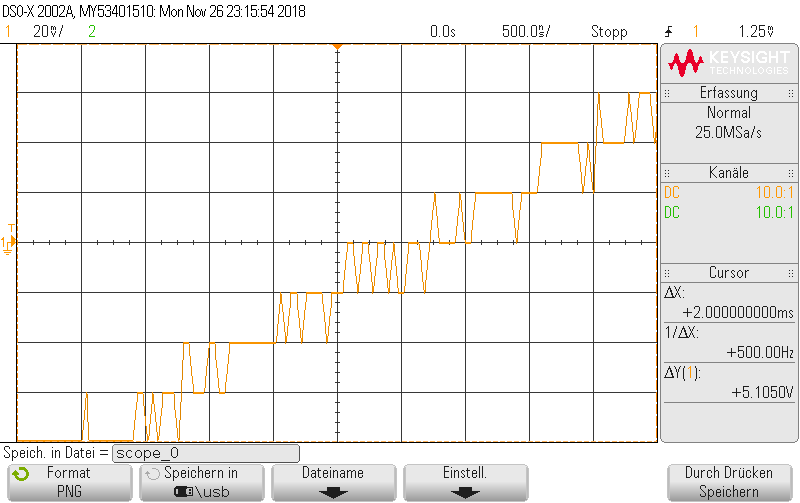
\includegraphics[width=0.8\textwidth]{./img/ch1/aufloesung}
  \caption{Quantisierungskennlinie}  
\end{figure} 
~\\

\subsection{Dynamik}
~\\
\begin{figure}[h]
  \centering
  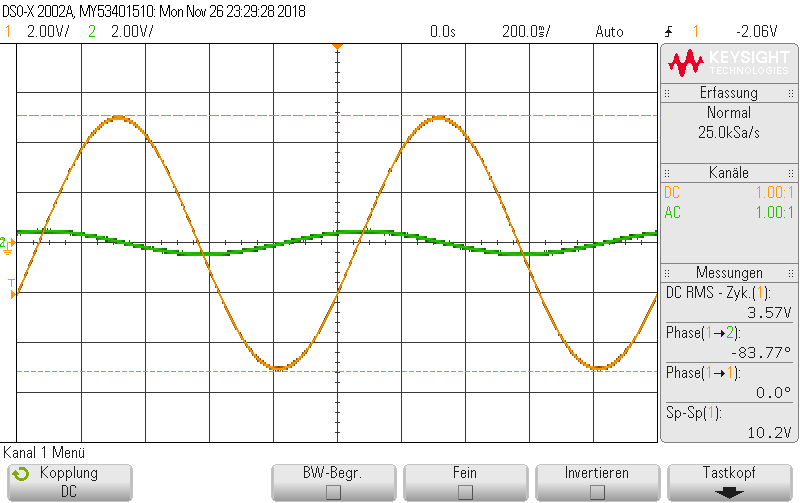
\includegraphics[width=0.8\textwidth]{./img/ch1/dynamik}
  \caption{Dynamik des Oszilloskops bei unterschiedlichen Eingangskopplungen}  
\end{figure} 
~\\

\subsection{Einschaltvorgang}
~\\
\begin{figure}[h]
  \centering
  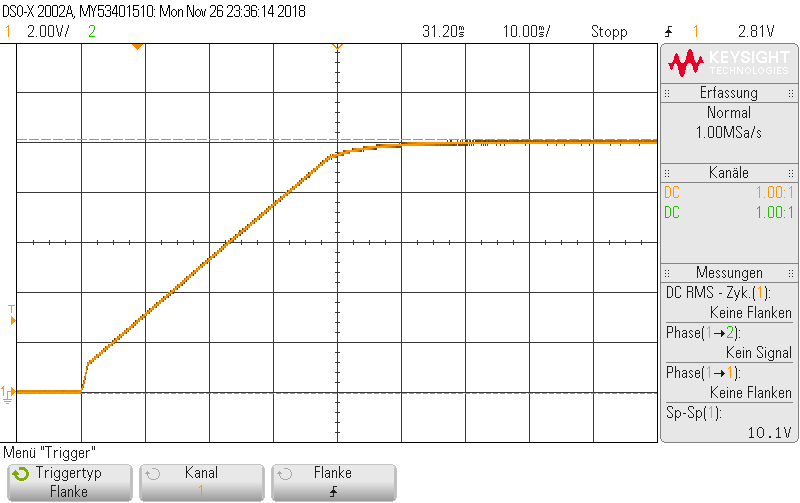
\includegraphics[width=0.8\textwidth]{./img/ch1/einschaltvorgang}
  \caption{Einschaltvorgang der Spannungsversorgung}  
\end{figure} 
~\\


